\documentclass[a4paper, 12pt, english]{article}

% \usepackage[portuges]{babel}
\usepackage[utf8]{inputenc}
\usepackage{amsmath,amssymb}
\usepackage{graphicx}
\usepackage{subfig}
\usepackage[colorinlistoftodos]{todonotes}

\usepackage{indentfirst}
\usepackage{verbatim}
\usepackage{textcomp}
\usepackage{gensymb}

\usepackage{relsize}

\usepackage{lipsum}% http://ctan.org/pkg/lipsum
\usepackage{xcolor}% http://ctan.org/pkg/xcolor
\usepackage{xparse}% http://ctan.org/pkg/xparse
\NewDocumentCommand{\myrule}{O{1pt} O{2pt} O{black}}{%
	\par\nobreak % don't break a page here
	\kern\the\prevdepth % don't take into account the depth of the preceding line
	\kern#2 % space before the rule
	{\color{#3}\hrule height #1 width\hsize} % the rule
	\kern#2 % space after the rule
	\nointerlineskip % no additional space after the rule
}
\usepackage[section]{placeins}

\usepackage{booktabs}
\usepackage{colortbl}%
\newcommand{\myrowcolour}{\rowcolor[gray]{0.925}}

\usepackage[obeyspaces]{url}
\usepackage{etoolbox}
\usepackage[colorlinks,citecolor=black,urlcolor=blue,bookmarks=false,hypertexnames=true]{hyperref}

\usepackage{geometry}
\geometry{
	paper=a4paper, % Change to letterpaper for US letter
	inner=3cm, % Inner margin
	outer=3cm, % Outer margin
	bindingoffset=.5cm, % Binding offset
	top=2cm, % Top margin
	bottom=2cm, % Bottom margin
	%showframe, % Uncomment to show how the type block is set on the page
}
\usepackage{fancyhdr}

% Define header and footer
\pagestyle{fancy}
\fancyhf{}
\lhead{ENER 104L}
\rhead{iSciM, Habib University} % Right-aligned page number in the header
\rfoot{\thepage} % Right footer text
%*******************************************************************************%
%************************************START**************************************%
%*******************************************************************************%
\begin{document}

%************************************TITLE PAGE**************************************%
\begin{titlepage}
	\begin{center}
		\textbf{\LARGE Habib University}\\[0.5cm]
		\textbf{\large iSciM}\\[0.2cm]
		\textbf {\large Fall 2023}\\[0.2cm]
		\vspace{20pt}
		
\includegraphics[width=5cm]{habiblogo.jpg}\\[1cm]
		\par
		\vspace{20pt}
		\textbf{\Large ENER 104L RENEWABLE ENERGY}\\
		\vspace{15pt}
		\myrule[1pt][7pt]
		\textbf{\LARGE  LABORATORY REPORT 1}\\
		\vspace{15pt}
		\textbf{\large Lab Name}\\
		\myrule[1pt][7pt]
		\vspace{25pt}
		\begin{tabular}{@{}p{5cm}p{3cm}@{}}
			\textbf{\large Student Name} & \textbf{\large Student ID} \\
			Ali Asghar Yousuf            & ay06993                    \\ % No1 
			Syed Ibrahim Ali Haider      & sh06565                    \\ % No2
		\end{tabular}

		\vspace{10pt}
		\begin{tabular}{@{}p{5cm}p{3cm}@{}}
			\textbf{\large Group Name} & \textbf{\large Group No.} \\
			Insane Fr                  & 1                         \\
		\end{tabular}

		\vspace{45pt}
		\textbf {\large Lab Instructors:}\\[0.2cm]
		\Large {Paishwa Naqvi}\\[0.1cm]
		\Large {Amber Talat}\\[0.1cm]
	\end{center}

	\par
	\vfill
	\begin{center}
		\textbf{\today}\\
	\end{center}

\end{titlepage}

%************************************TABLE OF CONTENTS**************************************%

%  %Sumário
%  \newpage
%  \tableofcontents
%  \thispagestyle{empty}
%  %End Sumário

%********************************%
%***********SECTION 1************%
%********************************%
\newpage
\section{Objectives}
abc

\section{Abstract}
Abstract

\section{Result and Analysis}
abc

\section{Conclusion}
abc

\section{Questions}

\section{Introduction}
The process of sending, propagating and receiving an analogue or digital
information signal over a physical point-to-point or point-to-multipoint
transmission medium, either wired, optical fiber or wireless is called
transmission. A distortion is defined as the alteration of the original shape
of an object, image, sound, waveform or other form of information or
representation. Distortion is usually unwanted, and often many methods are
employed to minimize it in practice. \newline

In this experiment, we are dealing with frequency response of RC circuit.
Frequency response is defined as the analysis of circuit with different
frequency of a sinusoidal source. With the sinusoidal source, the transfer
function, $H(s)$ will be the magnitude and phase of output voltage to the
magnitude and phase of input voltage of a circuit :

\begin{gather*}
	H(s) = \frac{V_o(s)}{V_i(s)}\\
\end{gather*}

The circuit in Figure~\ref{fig:Lowpass} is a first order low pass filter
circuit. First order is defined as 1 pair of resistor and capacitor connected
in series in a circuit. A low pass filter attenuates high frequency signal
input and only allows low frequency which below the cut-off frequency to pass
through. Cut-off frequency is the frequency filter start to attenuate the
passage of the input signals: $f_c = 2\pi RC$. At low frequncy, the reactance
of capacitor is high and the resistance is low. This result the voltage
potential across the capacitor is higher than voltage drop across the resistor.
Therefore, high frequency signals are attenuated in the experiment. \newline

The circuit in Figure~\ref{fig:Highpass} is acting as second order high pass
filter which is oppose to the meaning of low pass filter. High pass filter
passes signals above the cut-off frequency and attenuates low frequency
signals. By reversing the roles of resistors and capaciors, the reactance of
capacitors are low at high frequency signals. Therefore, the capacitors in the
circuit act as open circuit and attenuate low frequency input signals until
cut-off frequency reached. \newline

In last part of this experiment, we are studying the multipath propagation as
show in Figure~\ref{fig:Multipath}. Multipath occurs when a signal takes more
than one path from the transmitting antenna to the receiving antenna. Regarding
to lecture notes, the signals are received in a terrestrial environment, i.e.
where reflections are present and signals arrive at the receiver from the
transmitter via a variety of paths. The overall signal at the radio receiver is
a summation of the variety of signals being received. As they all have
different path lengths, the signals will add and subtract from the total
dependent upon their relative phases. Sometimes these will be in phase with the
main signal and will add to it, increasing its strength. At other times they
will interfere with each other. This will result in the overall signal strength
being reduced.

%********************************%
%***********SECTION 2************%
%********************************%
\newpage
\section{Objectives and Learning Outcomes}
\begin{enumerate}
	\item Distortion of signal during transmission occurs if the frequency response of
	      the transmission channel is not of constant amplitude and linear phase. In this
	      laboratory work, the student will:

	      \begin{enumerate}
		      \item Design and conduct an experiment to analyse the frequency, amplitude and phase
		            responses of a RC transmission line model.
		      \item Conduct an experiment to demonstrate the frequency sensitive fading phenomenon
		            using a simple two-path model of multi-path propagation.
	      \end{enumerate}
	\item To understand some factors that may cause signal transmission distortion, and
	      be motivated to study further other factors such as non-linearity, load
	      mismatching, time variant transmission medium properties and Gaussian noise.
\end{enumerate}

%********************************%
%***********SECTION 3************%
%********************************%

\section{Equipments}

\begin{itemize}
	\item  Breadboard, two 100 Ohm resistors, two 51 Ohm resistors, and three 10 k Ohm
	      resistors, four 1µF capacitors and three µ741 Op-Amp.
	\item  DC power supply, Function generator, Oscilloscope and Digital multi- meter.
\end{itemize}

%********************************%
%***********SECTION 4************%
%********************************%

\section{Methodology}

%***********************************************SUBSECTION 1************************************************%
\subsection{Frequency Response Measurement}

%*******************SUBSUBSECTION 1******************%     
\subsubsection{Part 1}

\begin{enumerate}
	\item An experiment was designed to study the amplitude and frequency response of the
	      circuit shown in Figure ~\ref{fig:Lowpass}.
	\item Data collected was recorded in an appropriate format. The results were analysed
	      and interpreted.
\end{enumerate}
\begin{figure}[!ht]
	\begin{center}
		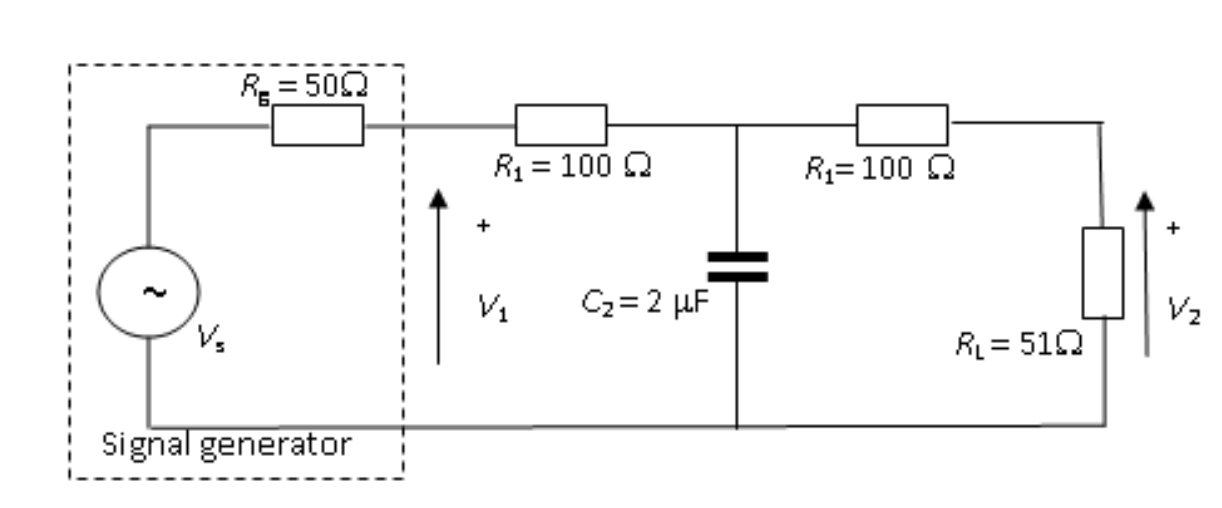
\includegraphics[width=100mm,scale=0.5]{Lowpass.png}
	\end{center}
	\caption{\label{fig:Lowpass}RC circuit(Low pass filter)}
\end{figure}

%*******************SUBSUBSECTION 2******************%

\subsubsection{Part 2}

\begin{enumerate}
	\item A 100 Hz square wave was applied to the input and the effect on the output
	      waveform $V_2$ was observed.
	\item Repeated with 1kHz follow by 10 kHz square wave.
	\item The observations were analysed and interpreted.
\end{enumerate}

%*******************SUBSUBSECTION 3******************%   
\subsubsection{Part 3}
\begin{enumerate}
	\item The changes in the results obtained in Part 2 were discussed if the circuit
	      shown in Figure~\ref{fig:Lowpass} is replaced with circuit shown in
	      Figure~\ref{fig:Highpass} below:
\end{enumerate}
\begin{figure}[!ht]
	\begin{center}
		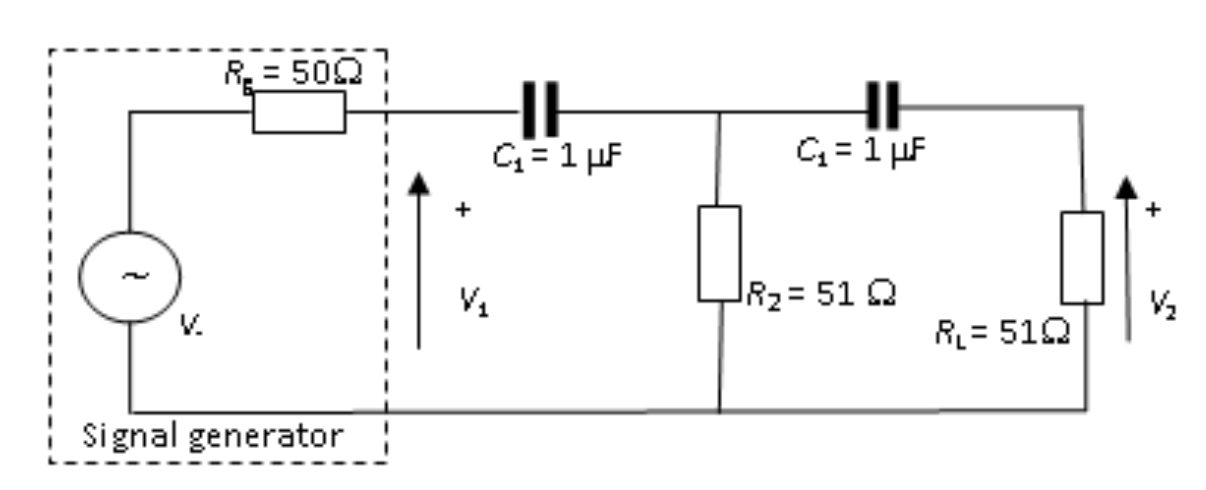
\includegraphics[width=100mm,scale=0.5]{Highpass.png}
	\end{center}
	\caption{\label{fig:Highpass}CR circuit(High pass filter)}
\end{figure}

%***********************************************SUBSECTION 2************************************************%

\subsection{Fading due to Multipath Propagation}

\begin{enumerate}
	\item $V_s$ was set to sine wave, frequency 500 Hz and Amplitude 10 volts, the waveform $V_2$ was sketched and  its amplitude was recorded.
	\item Repeated for frequencies 1, 1.5, 3 and 5 kHz and identify the frequency that
	      results in fading.
\end{enumerate}

\begin{figure}[!ht]
	\begin{center}
		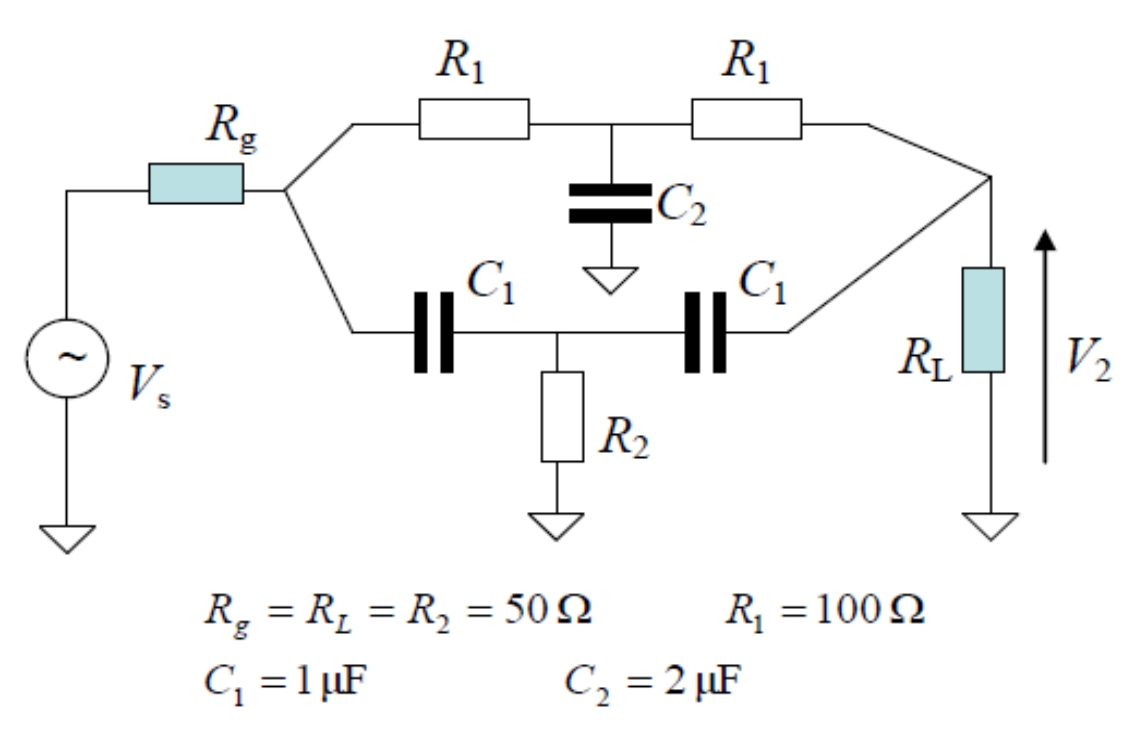
\includegraphics[width=100mm,scale=0.5]{Multipath.png}
	\end{center}
	\caption{\label{fig:Multipath}Multipath circuit(Band pass filter)}
\end{figure}

%********************************%
%***********SECTION 5************%
%********************************%
\null\newpage
\section{Result}

%***********************************************SUBSECTION 1************************************************%

\subsection{Frequency Response Measurement for RC circuit(Low pass filter)}

%*******************SUBSUBSECTION 1******************%
\subsubsection{Experimental Result}
%****************************************Table 1******************************************%
\begin{table}[!ht]
	\caption{\label{tab:Table 1} Experimental result for Second order low pass filter}
	\centering
	\begin{tabular}{c c c c c}
		\toprule
		\textbf{$ V_{in} (mV)$}
		     & \textbf{$ f $}
		     & \textbf{$V_{2} (mV)$}
		     & \textbf{(I.L)dB}
		     & \textbf{Phase ($\phi $)}                                   \\
		\cmidrule[0.4pt](r{0.125em}){1-1}%
		\cmidrule[0.4pt](lr{0.125em}){2-2}%
		\cmidrule[0.4pt](lr{0.125em}){3-3}%
		\cmidrule[0.4pt](lr{0.125em}){4-4}%
		\cmidrule[0.4pt](lr{0.125em}){5-5}%
		% \midrule
		5760 & 100 Hz                   & 1190   & -13.70 & $-5^{\circ}$  \\
		\myrowcolour%
		5730 & 200 Hz                   & 1160   & -13.87 & $-11^{\circ}$ \\
		5630 & 500 Hz                   & 1070   & -14.42 & $-21^{\circ}$ \\
		\myrowcolour%
		5320 & 1 kHz                    & 849    & -15.94 & $-38^{\circ}$ \\
		4930 & 2 kHz                    & 560    & -18.89 & $-65^{\circ}$ \\
		\myrowcolour%
		4830 & 5 kHz                    & 265.1  & -25.21 & $-74^{\circ}$ \\
		4780 & 10 kHz                   & 123.86 & -31.73 & $-77^{\circ}$ \\
		\myrowcolour%
		4700 & 20 kHz                   & 32.55  & -43.19 & $-79^{\circ}$ \\
		4700 & 50 kHz                   & 7.7    & -55.7  & $-83^{\circ}$ \\
		\myrowcolour%
		4700 & 100 kHz                  & 2.29   & -63.26 & $-85^{\circ}$ \\
		\bottomrule                                                       \\
	\end{tabular}
\end{table}
\begin{figure}[!ht]
	\begin{center}
		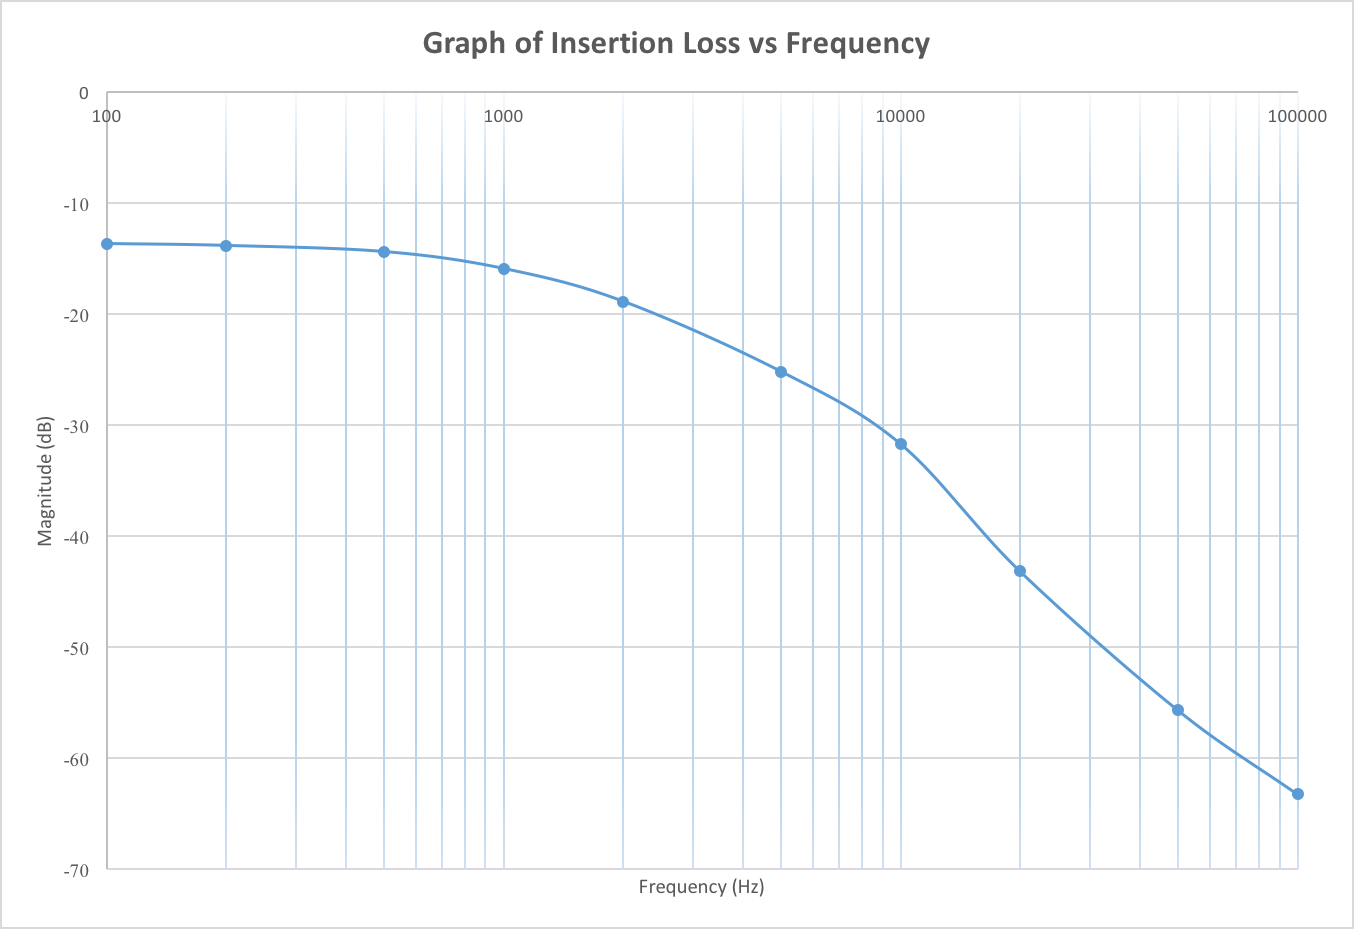
\includegraphics[width=140mm,scale=0.5]{P1_fr.png}
		\caption{\label{fig:P1_fr}Graph of insertion loss versus frequencies (Low pass filter)}
	\end{center}
\end{figure}
\begin{figure}[!ht]
	\begin{center}
		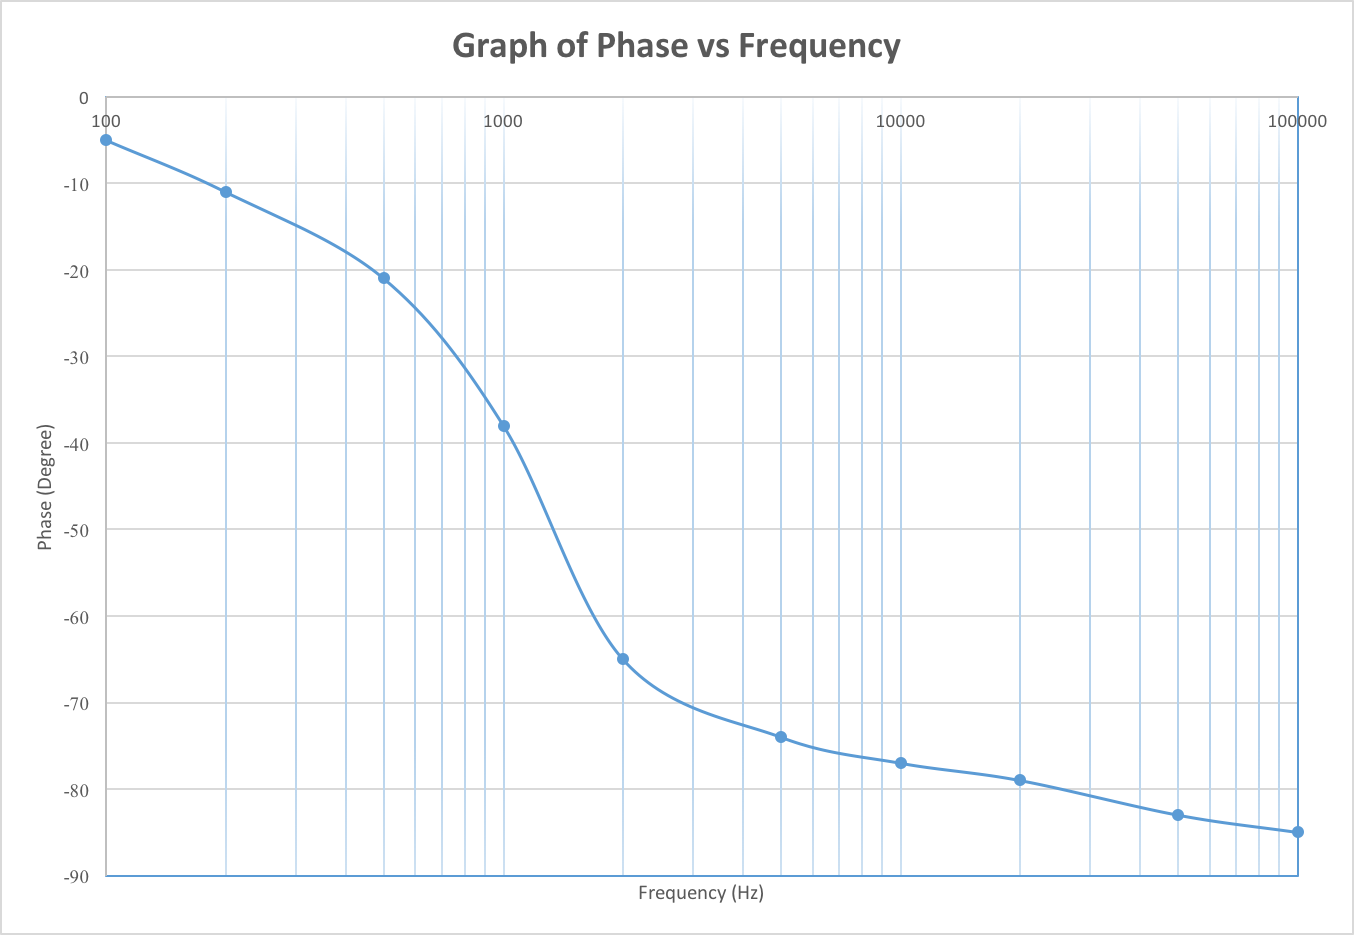
\includegraphics[width=140mm,scale=0.5]{P1_pr.png}
		\caption{\label{fig:P1_pr}Graph of phase versus frequencies (Low pass filter)}
	\end{center}
\end{figure}
\FloatBarrier
%****************************************   END  ******************************************%
%*******************SUBSUBSECTION 2******************%
\subsubsection{Transmission distortion over a RC channel}
\begin{figure}[!ht]
	\centering
	\subfloat[frequency = 100Hz]{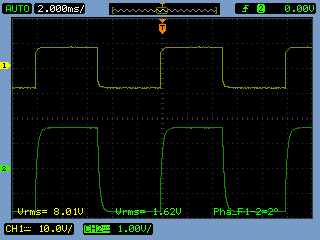
\includegraphics[width=0.4\columnwidth]{LPF100.png}}
	\qquad
	\subfloat[frequency = 1kHz]{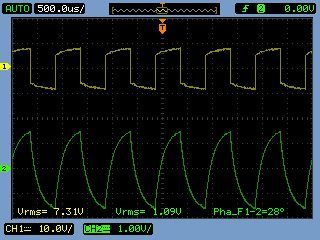
\includegraphics[width=0.4\columnwidth]{LPF1k.png}}
	\qquad
	\subfloat[frequency = 10kHz]{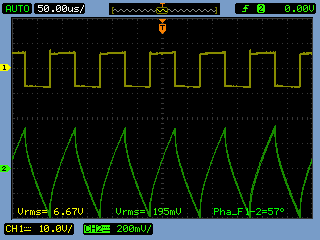
\includegraphics[width=0.4\columnwidth]{LPF10k.png}}
	\caption{Signal Transmission Distortion for LPF}
	\label{fig:STDLPF}
\end{figure}

%***********************************************SUBSECTION 2************************************************%
\newpage
\subsection{Frequency Response Measurement for the CR circuit(High pass filter)}
%*******************SUBSUBSECTION 1******************%
\subsubsection{Experimental Result}
%************************************Table 1**************************************%
\begin{table}[!ht]
	\caption{\label{tab:Table 2} Experimental result for Second order low pass filter}
	\centering
	\begin{tabular}{c c c c c}
		\toprule
		\textbf{$ V_{in} (mV)$}
		     & \textbf{$ f $}
		     & \textbf{$V_{2} (mV)$}
		     & \textbf{(I.L)dB}
		     & \textbf{Phase ($\phi $)}                                   \\

		\cmidrule[0.4pt](r{0.125em}){1-1}%
		\cmidrule[0.4pt](lr{0.125em}){2-2}%
		\cmidrule[0.4pt](lr{0.125em}){3-3}%
		\cmidrule[0.4pt](lr{0.125em}){4-4}%
		\cmidrule[0.4pt](lr{0.125em}){5-5}%
		% \midrule
		7310 & 100 Hz                   & 14.19  & -54.24 & $173^{\circ}$ \\
		\myrowcolour%
		7040 & 200 Hz                   & 40.0   & -44.91 & $164^{\circ}$ \\
		6720 & 500 Hz                   & 170.0  & -31.94 & $151^{\circ}$ \\
		\myrowcolour%
		6430 & 1 kHz                    & 492.85 & -22.31 & $131^{\circ}$ \\
		5370 & 2 kHz                    & 1050   & -14.18 & $108^{\circ}$ \\
		\myrowcolour%
		3920 & 5 kHz                    & 1840   & -6.57  & $72^{\circ}$  \\
		3180 & 10 kHz                   & 2040   & -3.86  & $45^{\circ}$  \\
		\myrowcolour%
		2840 & 20 kHz                   & 2170   & -2.34  & $25^{\circ}$  \\
		2530 & 50 kHz                   & 2200   & -1.21  & $12^{\circ}$  \\
		\myrowcolour%
		2580 & 100 kHz                  & 2230   & -1.27  & $7^{\circ}$   \\
		\bottomrule                                                       \\
	\end{tabular}
\end{table}
\begin{figure}[!ht]
	\begin{center}
		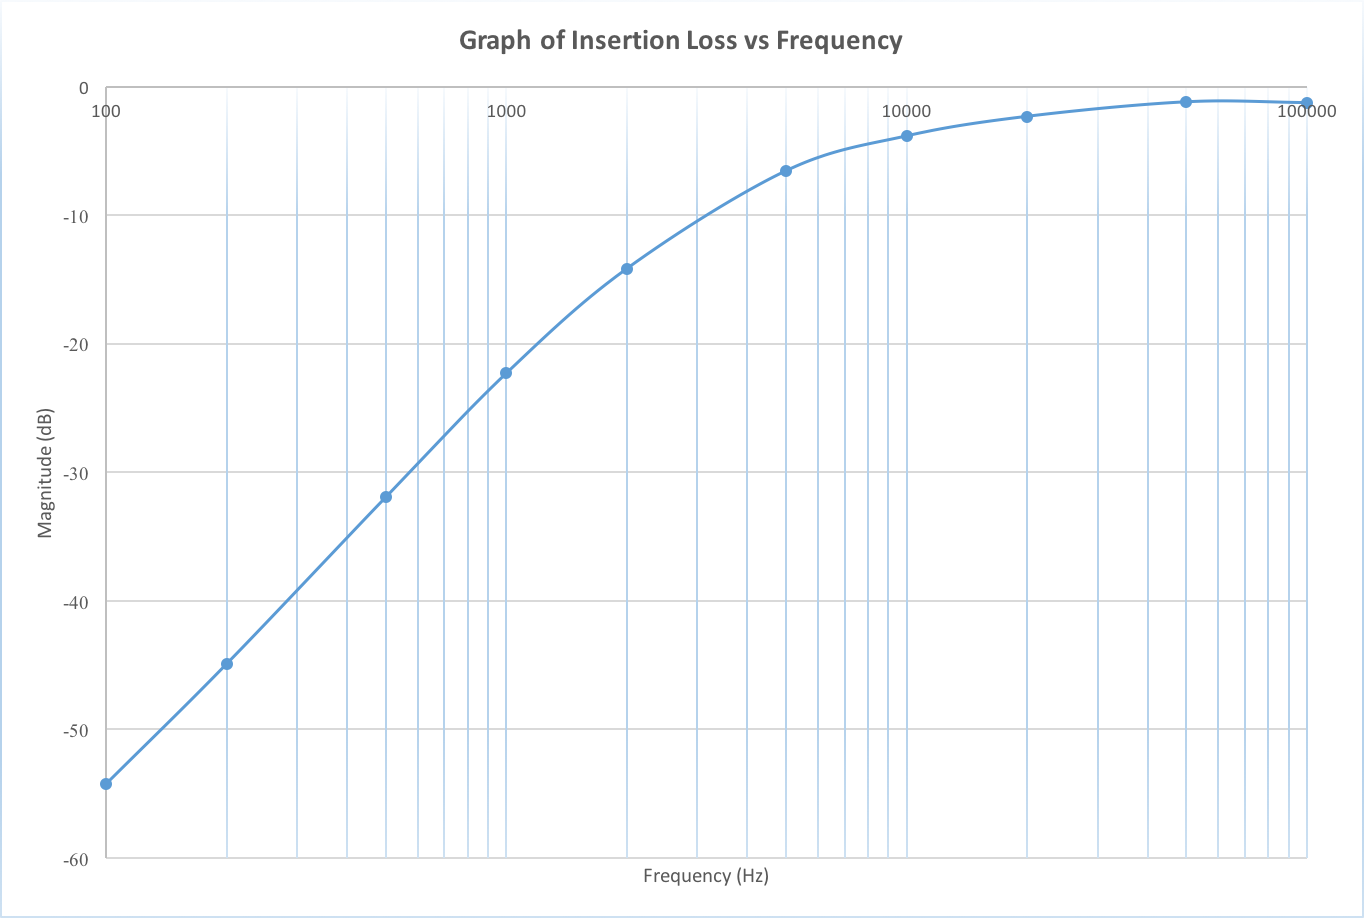
\includegraphics[width=140mm,scale=0.5]{P2_fr.png}
		\caption{\label{fig:P2_fr}Graph of insertion loss versus frequencies (High pass filter)}
	\end{center}
\end{figure}
\begin{figure}[!ht]
	\begin{center}
		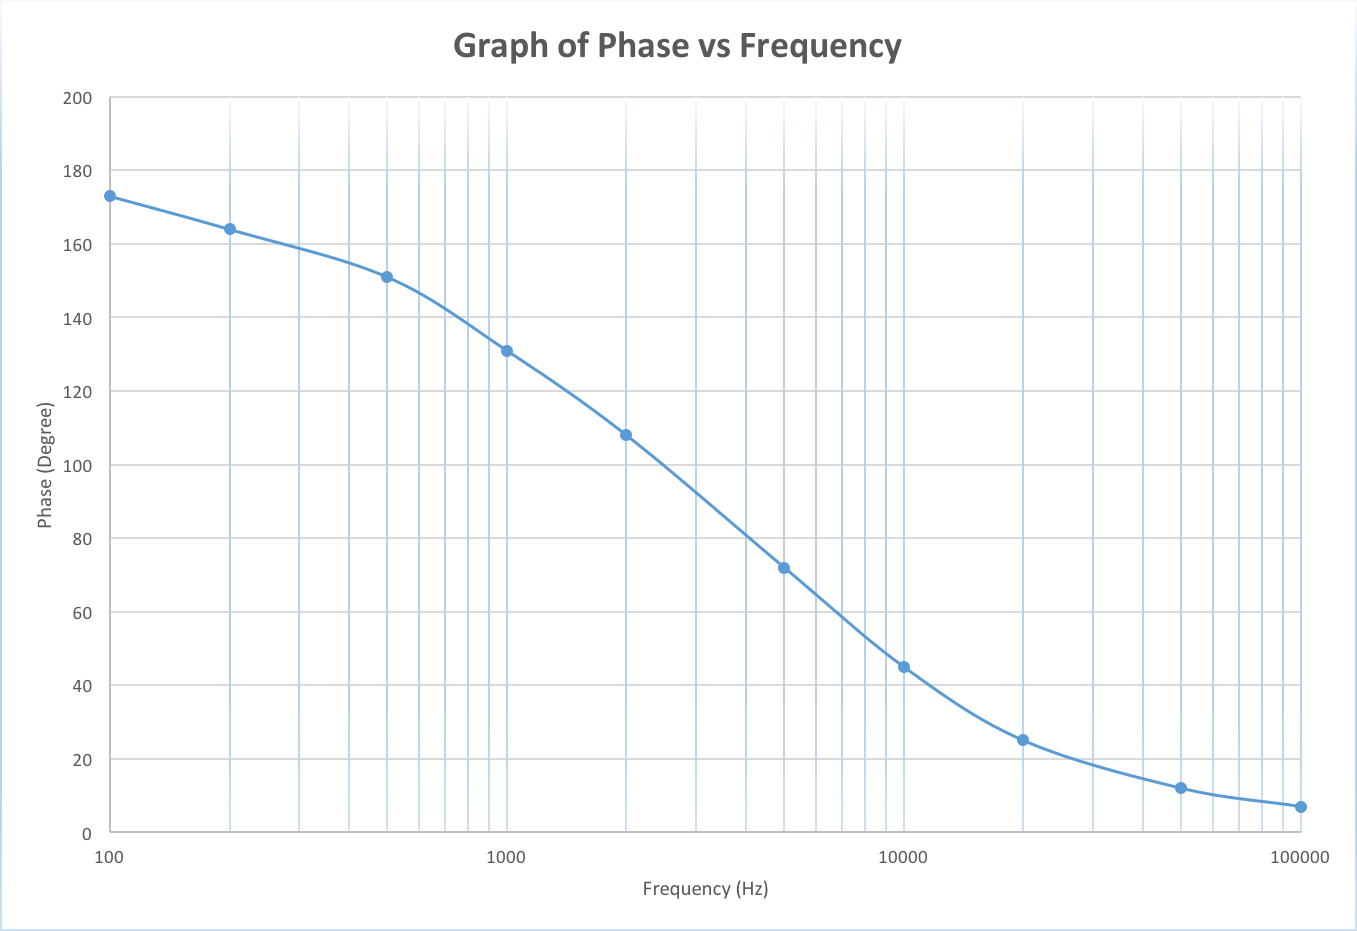
\includegraphics[width=140mm,scale=0.5]{P2_pr.png}
		\caption{\label{fig:P2_pr}Graph of phase versus frequencies (High pass filter)}
	\end{center}
\end{figure}
\FloatBarrier
%****************************************   END  ******************************************%
%*******************SUBSUBSECTION 2******************%
\subsubsection{Transmission distortion over a CR channel}

\begin{figure}[!ht]
	\centering
	\subfloat[frequency = 100Hz]{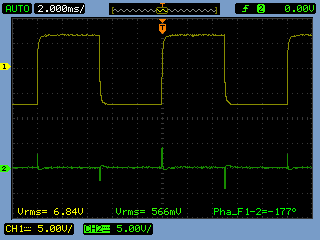
\includegraphics[width=0.4\columnwidth]{HPF100.png}}
	\qquad
	\subfloat[frequency = 1kHz]{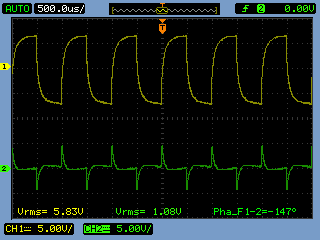
\includegraphics[width=0.4\columnwidth]{HPF1k.png}}
	\qquad
	\subfloat[frequency = 10kHz]{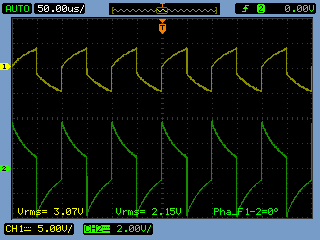
\includegraphics[width=0.4\columnwidth]{HPF10k.png}}
	\caption{Signal Transmission Distortion for HPF}
	\label{fig:STDHPF}
\end{figure}

%***********************************************SUBSECTION 3************************************************%

\subsection{Frequency Response Measurement for Fading due to Multipath Propagation (Band pass filter)}

%*******************SUBSUBSECTION 1******************%
\subsubsection{Experimental Result}
%************************************Table 1**************************************%
\begin{table}[!ht]
	\caption{\label{tab:Table 3} Experimental result for Multipath Propagation (Band pass filter)}
	\centering
	\begin{tabular}{c c c}
		\toprule
		\textbf{$ f $}
		        & \textbf{$V_{2} (mV)$}
		        & \textbf{(I.L)dB}               \\

		\cmidrule[0.4pt](r{0.125em}){1-1}%
		\cmidrule[0.4pt](lr{0.125em}){2-2}%
		\cmidrule[0.4pt](lr{0.125em}){3-3}%

		% \midrule
		500 Hz  & 1520                  & -13.27 \\
		\myrowcolour%
		1000 Hz & 1320                  & -14.49 \\
		1200 Hz & 1260                  & -14.89 \\
		\myrowcolour%
		1400 Hz & 1120                  & -15.92 \\
		1600 Hz & 1280                  & -14.76 \\
		\myrowcolour%
		1800 Hz & 1310                  & -14.56 \\
		2000 Hz & 1450                  & -13.67 \\
		\myrowcolour%
		2500 Hz & 1490                  & -13.44 \\
		3000 Hz & 1510                  & -13.32 \\
		\myrowcolour%
		5000 Hz & 1650                  & -12.55 \\
		\bottomrule                              \\
	\end{tabular}
\end{table}
\begin{figure}[!ht]
	\begin{center}
		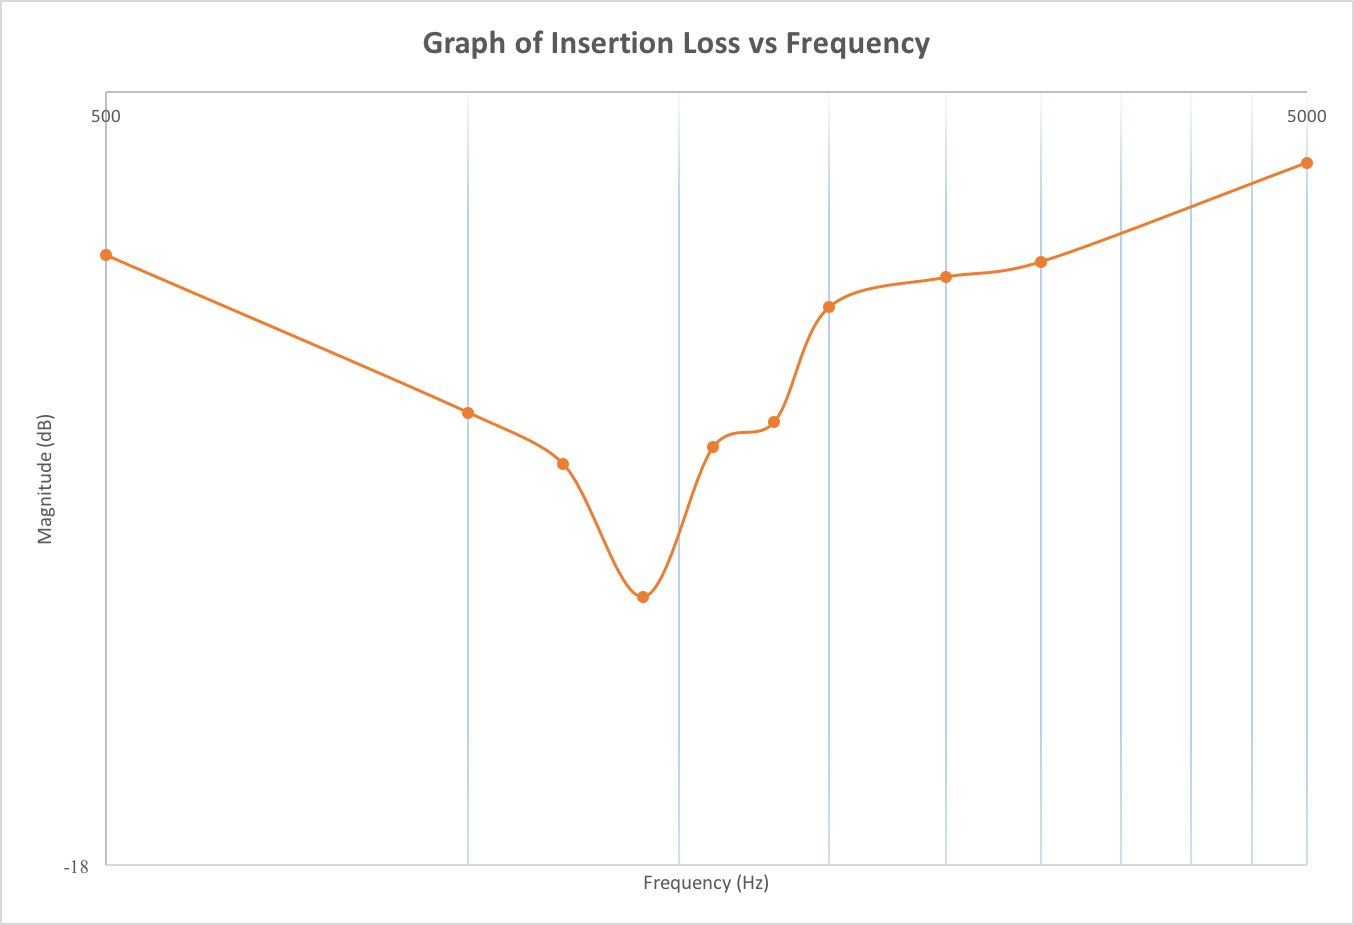
\includegraphics[width=140mm,scale=0.5]{P3_fr.png}
		\caption{\label{fig:P3_fr}Graph of insertion loss versus frequencies (Band pass filter)}
	\end{center}
\end{figure}
\FloatBarrier
%********************************%
%***********SECTION 6************%
%********************************%
\newpage
\section{Discussion}
A signal transmission system is the electrical channel between an information
source and destination. Signal transmission distortion can be divided into
amplitude distortion and frequency distortion. Linear distortion includes any
amplitude or delay distortion associated with a linear transmission system.
Amplitude distortion is easily described in the frequency domain; it means
simply that the output frequency components are not in correct proportion.
Since this is caused by $H(f)$ not being constant with frequency, amplitude
distortion is sometimes called frequency distortion. The most common forms of
amplitude distortion are excess attenuation or enhancement of extreme high or
low frequencies in the signal spectrum. While the frequency-domain description
is easy, the effects in the tie domain are far less obvious, except for very
simple signals. The loss of the high-frequency term reduces the “sharpness” of
the waveform. The “flat” frequency response means that the frequency range over
which $|H(f)|$ must be constant to within a certain tolerance so that the
amplitude distortion is sufficiently small.

\subsection{Part1}
For the part 1 of the experiment, we are dealing with the frequency response
for a RC circuit which is also a first order low pass filter. The low pass
filter only allows low frequency signals from 0Hz to its cut-off frequency,
$f_{c}$ point to pass while blocking those any higher. The circuit shown in
Figure~\ref{fig:Lowpass} uses two passive first-order low pass filters
connected or “cascaded” together to form a second-order or two-pole filter
network. Hence, we can see that a first-order low pass filter can be converted
into a second-order type by simply adding an additional RC network to it and
the more RC stages we add the higher becomes the order of the filter. As the
order of the filter is increased, the roll-off slope becomes steeper and the
actual stop band response of the filter approaches its ideal stop band
characteristics \cite{LPF}. \newline

Based on the Table~\ref{tab:Table 1}, we obtained that the range of insertion
loss from -13.70dB to -63.26dB which is decreasing as the frequency increasing.
The frequency response and phase response of the low pass circuit were show in
Figure~\ref{fig:P1_fr} and Figure~\ref{fig:P1_pr} respectively. The result from
the Frequency Response graph shows that the insertion loss decreases gradually
as the frequency is increasing. Regarding to the Phase Response graph plotted,
the degree of phase decreases as the frequency increases. The Frequency
Response of the filter to be nearly flat for low frequencies until it reaches
its Cut-off Frequency point $(f_{c})$. This is because the reactance of the
capacitor is high at low frequencies and blocks any current flow through the
capacitor. We obtained the cutoff frequency at -16.7dB (-13.7dB-3dB) which are
1100Hz experimental result. The phase shift for experimental result is
$-43^{\circ}$. \newline

Following, we have observed the transmission distortion for the RC circuit for
different values of frequencies. The integrator is basically a low pass filter
circuit operating in the time domain that converts a square wave “step”
response input signal into a triangular shaped waveform output as the capacitor
charges and discharges. A triangular waveform consists of alternate but equal,
positive and negative ramps. From observation on the output waveform as show as
Figure~\ref{fig:STDLPF}, the output become more triangle in shape as the
frequency of the input signal increase. This is because of the exponential
charging and discharging processes of the capacitor cause the triangular
waveform at output. As our input waveform is square wave, it consists of
summation of odd harmonic of sinusoid. Since LPF attenuates high frequency
components, the summation of low frequency of odd harmonic sinusoid give rise
to the triangle shape of output waveform.

\subsection{Part2}
In part 2 of the experiment, we are dealing with the frequency response for a
CR circuit which is also a second order high pass filter. The high pass filter
only allows high frequency signals from its cut-off frequency, $f_{c}$ point
and higher to infinity to pass through while blocking those any lower. The
circuit shown in Figure~\ref{fig:Highpass} uses two first-order high pass
filters connected or cascaded together to form a second-order or two-pole high
pass network. \newline

Based on the Table~\ref{tab:Table 2}, we obtained that the range of insertion
loss from -54.24dB to -1.27dB which is increasing as the frequency increasing.
The frequency response and phase response of the high pass circuit were show in
Figure~\ref{fig:P2_fr} and Figure~\ref{fig:P2_pr} respectively. The result
Frequency Response graph shows a positive relationship between the insertion
loss and the frequency. The insertion loss increases as the frequency
increases. Whereas for the Phase Response graph, the degree of phase decreases
as the frequency increases. Frequency Response for high pass filter is the
exact opposite to that of a low pass filter. It has a response curve that
extends down from infinity to the cut-off frequency. We obtained the cutoff
frequency at -4.27dB (-1.27dB-3dB) which are 10000Hz experimental result. Also
we can see that the phase angle $(\phi)$ of the output signal LEADS that of the
input and is equal to $+46^{\circ}$ for experimental result at frequency
$f_{c}$. \newline

Thereafter, we have observed the transmission distortion for the CR circuit for
different values of frequencies. If we change the input signal to that of a
“square wave” shaped signal that has an almost vertical step input, the
response of the circuit changes dramatically and produces a circuit known
commonly as a Differentiator. However, if we feed the High Pass Filter with a
Square Wave signal operating in the time domain giving an impulse or step
response input, the output waveform will consist of short duration pulse or
spikes as shown in Figure~\ref{fig:STDHPF}. Each cycle of the square wave input
waveform produces two spikes at the output, one positive and one negative and
whose amplitude is equal to that of the input. The rate of decay of the spikes
depends upon the time constant, (RC) value of both components, (t = R x C) and
the value of the input frequency. The output pulses resemble more and more the
shape of the input signal as the frequency increases.

\subsection{Part3}
In part 3 of the experiment, we have dealing with the fading due to the
multipath propagation. The circuit is actually a combination of first order low
pass filter and second order high pass filter to form a simple two-path model
of multipath propagation. As the input signal transmitted through the low pass
filter and high pass filter, each of the signal will be attenuated and cause
the phase shift by different amount. Hence, when the signals reach the load
resistance, the summation of each signal will cause interference and phase
shift of output signal which is known as multipath fading. ‘Fading’ means rapid
fluctuations of the amplitudes, phases or multipath delays of a radio signal
over a short period or short travel distance. This might be so severe that
large scale radio propagation loss effects might be ignored. The frequency
response is shown in Figure~\ref{fig:P3_fr}. From the Table~\ref{tab:Table 3},
the fading frequency is 1.4kHz because it has the lowest amplitude among the 10
frequencies. The results proved that the frequency 1.4kHz has the narrowest
bandwidth and allow minimum signal to pass through. \newline

Last but not least, there are some precautions that we should realize
throughout the experiment. The lesser number of wire are encouraged to avoid
any confusion when having circuit checking if any error occurs. Moreover, the
electrical devices and breadboard should be checked if its well-functioning
before using it to avoid any delay. Lastly, the polarity of the capacitor must
place correctly to avoid any accident happen.

%********************************%
%***********SECTION 7************%
%********************************%
\newpage
\section{Conclusion}
There are many factors may cause distortion in signal transmission. After
completion of the experiment, we understand some factors from experiment, which
are channel with insufficient bandwidth, multipath propagation channel and
fading channel. In the last part of this experiment, the frequency that caused
fading due to multipath propagation is 1.4kHz.

%********************************%
%***********SECTION 8************%
%********************************%

\patchcmd{\thebibliography}{\section*}{\section}{}{}
% Now we need a bibliography:
\begin{thebibliography}{99}

	%Each item starts with a \bibitem{reference} command and the details thereafter.
	\bibitem{LPF} % Web document
	Electronics Tutorials Low Pass Filter
	\url{http://www.electronics-tutorials.ws/filter/filter_2.html}.

	\bibitem{HPF} % Web document
	Electronics Tutorials High Pass Filter
	\url{http://www.electronics-tutorials.ws/filter/filter_3.html}.

	\bibitem{MVP} % Web document
	Multipath Wave Propagation
	and Fading
	\url{http://www.iitg.ernet.in/scifac/qip/public_html/cd_cell/chapters/a_mitra_mobile_communication/chapter5.pdf}.

	\bibitem{5}
	Frequency response of RC and LR circuits
	\url{http://www.ece.sunysb.edu/~oe/Leon/ESE211/Lab05}

\end{thebibliography}
\noindent
\end{document}